% =====================================================================
% main.tex -- the ONLY file that gets compiled.
%
% Build:
%   pdflatex main
%   bibtex   main
%   pdflatex main
%   pdflatex main
%
% Four passes, because LaTeX only learns page and citation numbers after
% the first one. "??" or "[?]" in the PDF just means: build again.
%
% ICLR 2027, double blind. \iclrfinalcopy stays COMMENTED OUT for the
% submission -- uncommenting it would print the author block and the
% paper would be desk rejected.
% =====================================================================

\documentclass{article}
\usepackage{iclr2027_conference,times}

% =====================================================================
% preamble.tex -- packages, macros and switches for the ICLR 2027 paper.
%
% Rule for this file: the official style files are NEVER edited. Anything
% we need goes here instead. The guidelines say tweaking the style files
% "may be grounds for rejection".
% =====================================================================

\usepackage{amsmath}
\usepackage{amssymb}
\usepackage{amsthm}
\usepackage{graphicx}
\usepackage{booktabs}
\usepackage{multirow}
\usepackage{subcaption}
\usepackage{xcolor}
\usepackage{microtype}

\usepackage{hyperref}
\usepackage{url}
\hypersetup{
  colorlinks = true,
  linkcolor  = black,
  citecolor  = black,
  urlcolor   = blue!60!black,
  % Double blind: no author name may leak through the PDF metadata (issue I1).
  pdfauthor  = {},
  pdfsubject = {},
  pdfkeywords= {}
}

% cleveref must be loaded AFTER hyperref, otherwise the links break.
\usepackage[capitalise,noabbrev]{cleveref}

% ---------------------------------------------------------------------
% Where images live. The paper sits two folders below the project root,
% so "../../" reaches results/ and the generated figures. No file
% extension is written in \includegraphics, so LaTeX picks the sharp PDF.
% ---------------------------------------------------------------------
\graphicspath{{../../}{figures/}}

% ---------------------------------------------------------------------
% Names we write over and over. One macro each, so a rename is one edit
% and spelling can never drift between sections.
% ---------------------------------------------------------------------
\newcommand{\seanet}{SEA-Net}
\newcommand{\millet}{MILLET}
\newcommand{\webtraffic}{WebTraffic}
\newcommand{\ucr}{UCR}
\newcommand{\ndcg}{NDCG@$n$}

% Anonymous code link. Replace the placeholder with the real anonymised
% mirror before submitting -- see issue I18 in PAPER_ISSUES.md.
\newcommand{\anonrepo}{\url{https://anonymous.4open.science/r/seanet-ANON}}

% ---------------------------------------------------------------------
% Notation. Defined once here, used everywhere, never redefined.
% ---------------------------------------------------------------------
\newcommand{\R}{\mathbb{R}}
\newcommand{\bag}{\mathbf{X}}              % the input series (the bag)
\newcommand{\inst}{x}                      % one time step (an instance)
\newcommand{\emb}{\mathbf{z}}              % embedding of one time step
\newcommand{\instpred}{\mathbf{y}}         % per-time-step class logits
\newcommand{\bagpred}{\hat{y}}             % bag logits (the prediction)
\newcommand{\interp}{\mathbf{I}}           % the interpretation
\newcommand{\nsteps}{T}                    % number of time steps
\newcommand{\nclz}{C}                      % number of classes
\newcommand{\dmodel}{d}                    % encoder width
\newcommand{\dattn}{d_a}                   % attention width
\newcommand{\sig}{\sigma}
\newcommand{\softmaxt}{\operatorname{softmax}_j}
\newcommand{\softplus}{\operatorname{softplus}}
\DeclareMathOperator*{\argmax}{arg\,max}

% ---------------------------------------------------------------------
% A "finding" environment, so the four claims of the paper look the same
% every time they appear and a reviewer can find them by skimming.
% ---------------------------------------------------------------------
\newtheorem{finding}{Finding}
\newtheorem{property}{Property}

% Compact list spacing -- pages are the scarce resource here (issue I9).
\usepackage{enumitem}
\setlist[itemize]{topsep=2pt,itemsep=1pt,parsep=0pt,leftmargin=1.4em}
\setlist[enumerate]{topsep=2pt,itemsep=1pt,parsep=0pt,leftmargin=1.6em}

% Slightly tighter floats, again for the page budget.
\setlength{\textfloatsep}{10pt plus 2pt minus 2pt}
\setlength{\intextsep}{10pt plus 2pt minus 2pt}
\setlength{\abovecaptionskip}{4pt}
\setlength{\belowcaptionskip}{2pt}


\title{Selection, Not Scale: What Controls Accuracy and\\
       Faithfulness in Inherently Interpretable\\
       Time Series Classification}

% Authors are hidden while \iclrfinalcopy is commented out. Do not put
% real names here -- the style file prints this block in final mode only,
% but a name left in the source can still leak through PDF metadata.
\author{Anonymous authors\\
Paper under double-blind review}

%\iclrfinalcopy   % <-- camera-ready ONLY. Never for the submission.

\begin{document}

\maketitle

\begin{abstract}
% !TEX root = ../main.tex
% =====================================================================
% ABSTRACT -- one paragraph, as the ICLR style requires.
% It must promise exactly the four findings and nothing more.
% =====================================================================

Inherently interpretable time series classifiers built on Multiple Instance Learning (MIL) return a
label and, from the same computation, an importance score for every time step. Progress in this
line is usually reported as a stronger backbone paired with a better faithfulness score. We ask a
different question: inside this family, what actually controls accuracy and explanation quality? We
train 72 encoder $\times$ pooling-head combinations under one identical configuration, on a dataset
with per-time-step ground truth and on 85 \ucr{} datasets, and report four findings. \textbf{(i)}
Explanation quality is governed by \emph{selection inside the aggregator} rather than by encoder
capacity: restricting the bag score to the largest $\kappa$ fraction of per-step evidence -- a head
that reduces \emph{exactly} to the standard conjunctive baseline at $\kappa = 1$ -- raises
ground-truth ranking quality from $0.722$ to $0.777$ \ndcg{}, and costs about one point of accuracy.
\textbf{(ii)} Faithful interpretability is cheap: a $41$\,K-parameter model matches or exceeds a
$424$\,K-parameter \millet{} baseline on accuracy, AOPCR and \ndcg{} \emph{simultaneously}, and the
residual gap on \ucr{} is a capacity effect, not an architectural one -- at comparable capacity our
encoder outranks the baseline ($11.53$ against $12.60$ mean rank). \textbf{(iii)} AOPCR, the
faithfulness metric this literature reports, is not comparable across training configurations: the
same architecture and the same code score $2.57$ under one recipe and $13.27$ under another, a
$5.2\times$ swing that no change in explanation quality accounts for. We show why, and give a
reporting protocol. \textbf{(iv)} Pooling heads that \emph{provably} contain the baseline as a
special case still fail badly in practice -- the worst head we test is one of them -- because
nothing in the objective drives the model back to the safe branch. Capacity-safety is not
optimisation-safety. Together these results suggest the aggregator, not the backbone, is where the
design effort in interpretable time series classification belongs.

\end{abstract}

% !TEX root = ../main.tex
% =====================================================================
% 1. INTRODUCTION -- page budget 1.25
%
% Written LAST, so it promises exactly what Sections 5-8 deliver and
% nothing more. Order: the setting -> the question nobody asked ->
% the four findings -> what we do not claim.
% =====================================================================

\section{Introduction}
\label{sec:intro}

A time series classifier that only returns a label is of limited use where someone has to act on
its output. When a model flags an anomaly in a patient recording or in a machine's vibration trace,
the operator needs to know \emph{which part of the signal} triggered the alert.
\citet{rudin2019stop} argues that in such settings a model that is interpretable \emph{by design}
should be preferred to a black box paired with a post-hoc explainer, because only the first
guarantees that the explanation and the decision are the same computation.

For time series, the leading realisation of that idea is Multiple Instance Learning (MIL). \millet{}
\citep{early2024millet} treats a series as a bag of time steps, replaces the global average pooling
that ends every standard convolutional classifier \citep{wang2017fcn, fawaz2020inceptiontime} with a
MIL \emph{pooling head} that scores each step, and computes the class prediction from those scores.
The scores are therefore the explanation and the prediction at once. Work in this line is normally
presented the same way: a backbone, a pooling head, an accuracy table, and a faithfulness score.

This paper asks a question that presentation leaves unanswered: \emph{within this family, what
actually controls accuracy and explanation quality?} The question is answerable because the family
factorises cleanly. A model is an encoder followed by a pooling head, the two communicate through
one fixed tensor interface, and either can be replaced without touching the other. We exploit that
to run a controlled sweep -- 72 encoder $\times$ pooling-head combinations, up to 129 datasets each,
every model trained under a single identical configuration, with the \millet{} baseline re-trained
inside the same harness rather than quoted from its paper. Under that design, any difference in the
results is attributable to the component we changed.

The sweep is built around \seanet{}, a compact multi-scale depthwise-separable encoder family and
seven MIL pooling heads, each head targeting a specific limitation of \millet{}'s conjunctive
pooling (\Cref{sec:design}). \seanet{} is the \emph{instrument} of this study rather than its
result: it exists so that capacity, aggregation rule and training budget can be varied
independently. Four findings follow, and they are the contribution of this paper.

\begin{itemize}
  \item \textbf{Selection inside the aggregator, not encoder capacity, drives explanation quality}
        (\Cref{sec:selection}). Averaging only the largest $\kappa$ fraction of per-step evidence
        makes the importance map exactly zero wherever the model used nothing. Because
        $\kappa = 1$ recovers the conjunctive baseline \emph{exactly}, sweeping $\kappa$ is a
        controlled experiment on selection alone: ground-truth ranking quality rises from $0.722$ to
        $0.777$ \ndcg{}, with an optimum rather than a monotone gain, and costs about one accuracy
        point. A second, independent knob -- an attention-entropy penalty -- moves both quantities
        the same way.

  \item \textbf{Faithful interpretability does not require a large backbone, and the residual gap is
        capacity} (\Cref{sec:cheap}). A $41$\,K-parameter model beats the $424$\,K-parameter
        baseline on accuracy, AOPCR and \ndcg{} at the same time on the one dataset where
        explanation correctness can be checked against ground truth. On the 85 \ucr{} datasets the
        small models fall behind the baseline, but a wider version of the \emph{same} encoder
        overtakes it ($11.53$ against $12.60$ mean rank), which locates the effect in capacity
        rather than in architecture.

  \item \textbf{AOPCR is not comparable across training configurations} (\Cref{sec:aopcr}). Holding
        the architecture, the code, the metric implementation and the data fixed and changing only
        the training recipe moves AOPCR from $2.57$ to $13.27$. AOPCR is an area over a curve of raw
        confidence differences, so its scale follows the scale of the logits. Every cross-paper
        AOPCR comparison in this literature is therefore uninterpretable, including comparisons
        against the published numbers of the method we build on. We give a reporting protocol that
        costs nothing to adopt.

  \item \textbf{Capacity-safety is not optimisation-safety} (\Cref{sec:safety}). Five of our seven
        heads provably reduce to the conjunctive baseline for one setting of their parameters, an
        argument used routinely to claim a design ``cannot hurt''. One of them is nonetheless the
        worst head we test, by a wide margin. The mechanism is identifiable: no term in the
        objective pushes the blend parameter back towards the safe branch, so a head that
        \emph{can} represent the baseline never finds it.
\end{itemize}

\paragraph{What we do not claim.}
We do not claim state of the art on the \ucr{} archive; we are not, and \Cref{sec:cheap} reports the
margin by which. We do not claim that the encoder variants we build are individually important --
\Cref{sec:cheap} shows the best pair is not composed of the two individually best halves. And
because of \Cref{sec:aopcr}, we do not compare any AOPCR value in this paper against an AOPCR
printed in another one. Every number we report was produced under a single configuration inside one
harness, and the code that produced it is available at \anonrepo{}.

% !TEX root = ../main.tex
% =====================================================================
% 2. BACKGROUND -- page budget 1.0
%
% Only what a reader needs to follow Sections 5-8: the MIL view, the
% baseline head we compare everything against, and the two metrics.
% The notation defined here is never redefined later.
% =====================================================================

\section{Background}
\label{sec:bg}

\subsection{Time series as bags of time steps}
\label{sec:bg:mil}

A univariate series $\bag = (\inst_1, \dots, \inst_{\nsteps})$ carries one label
$y \in \{1,\dots,\nclz\}$, but in most datasets only a few time steps hold the evidence for it. That
is exactly the structure of Multiple Instance Learning \citep{dietterich1997mil}, where a labelled
\emph{bag} contains unlabelled \emph{instances}: take the series as the bag and each time step as an
instance, and recovering the explanation becomes the standard MIL problem of recovering
instance-level contributions from a bag-level label.

An encoder maps every step to an embedding, $\emb_j = f_\theta(\bag)_j \in \R^{\dmodel}$, and a MIL
pooling head reduces the $\nsteps$ embeddings to a bag prediction $\bagpred \in \R^{\nclz}$.
Attention-based MIL \citep{ilse2018attention} learns how much each instance counts, and because the
attention weight is the quantity the prediction is built from, it can be read directly as an
importance score. The most active application of this idea is histopathology, where a slide is a bag
and a patch is an instance; two methods from that literature -- multi-scale fusion
\citep{hashimoto2020msdamil} and the dual-stream critical-instance mechanism of
\citet{li2021dsmil} -- are adapted to time series in \Cref{sec:design}.

\subsection{The baseline: conjunctive pooling}
\label{sec:bg:conj}

\millet{} \citep{early2024millet} pairs an InceptionTime encoder \citep{fawaz2020inceptiontime} with
\emph{conjunctive pooling}, which combines one attention gate with a per-time-step classifier:
\begin{equation}
  a_j = \sig\!\big(\mathbf{w}_a^\top \tanh(W_a \emb_j)\big) \in [0,1],
  \qquad
  \instpred_j = W_c \emb_j + \mathbf{b}_c \in \R^{\nclz},
  \label{eq:conj_gate}
\end{equation}
\begin{equation}
  \bagpred^{\,k} = \frac{1}{\nsteps}\sum_{j=1}^{\nsteps} a_j \instpred_j^{\,k},
  \qquad
  \interp_{k,j} = a_j \instpred_j^{\,k} .
  \label{eq:conj_bag}
\end{equation}
The interpretation $\interp_{k,j}$ is made of the same terms that are summed to give
$\bagpred^{\,k}$, so the explanation cannot disagree with the prediction: it \emph{is} the
prediction, decomposed. Three properties of \Cref{eq:conj_bag} bound what the head can express, and
each one motivates a family of heads in \Cref{sec:design}. \textbf{L1, one gate for all classes:}
$a_j$ is a single scalar per step, so a step cannot support one class while arguing against another.
\textbf{L2, weights not normalised over time:} the gate is a sigmoid and the sum is divided by
$\nsteps$, so the magnitude of $\bagpred^{\,k}$ depends on the series length -- awkward on an archive
whose lengths span $15$ to $2{,}844$. \textbf{L3, a fixed mean:} evidence concentrated in a few steps
of a long series contributes a vanishing share of the average, and a fixed operator cannot adapt to
datasets where the evidence is instead spread out.

\subsection{Measuring explanation quality}
\label{sec:bg:metrics}

We use the two metrics of \citet{early2024millet}, computed with their implementation, because our
purpose is to compare against their method on their own terms.

\paragraph{AOPCR (faithfulness to the model).}
Steps are ranked by the model's own interpretation, masked one at a time in that order, and the
confidence in the original prediction is tracked; a faithful ranking makes it fall fast. Writing
$O^k$ for the induced ranking and $\bag^{O^k}_j$ for the series with its $j$ most important steps
masked \citep{samek2017aopc},
\begin{equation}
  \mathrm{AOPC}(\bag, O^k) = \frac{1}{\nsteps-1}\sum_{j=1}^{\nsteps-1}
  \Big[\bagpred^{k}(\bag) - \bagpred^{k}\big(\bag^{O^k}_{j}\big)\Big],
  \label{eq:aopc}
\end{equation}
and AOPCR reports the margin of \Cref{eq:aopc} over three random maskings, so that a merely fragile
model is not rewarded. AOPCR needs no ground truth and is therefore available on every dataset. It
is also, as \Cref{sec:aopcr} shows, \textbf{unnormalised} -- it is built from raw confidence
differences, so its scale follows the scale of the logits.

\paragraph{\ndcg{} (correctness against ground truth).}
Normalised Discounted Cumulative Gain \citep{jarvelin2002ndcg} asks whether the steps that
\emph{genuinely} matter appear at the top of the ranking. It needs per-time-step ground truth, which
only a synthetic generator provides, but it is normalised to $[0,1]$ and is therefore the metric we
lean on whenever the two disagree.

% !TEX root = ../main.tex
% =====================================================================
% 3. THE DESIGN SPACE -- page budget 1.25
%
% This is the "method" section, but it is written as the axes of the
% study, not as a product pitch. Full equations for every head and every
% encoder variant are in Appendix B; here we give the two slots, the
% reduction properties (which is what makes the sweep controlled), and
% only the one head that Section 5 needs in closed form.
% =====================================================================

\section{The Design Space We Sweep}
\label{sec:design}

A model in this family is a pair \emph{encoder $+$ pooling head}. The encoder consumes
$(B,1,\nsteps)$ and returns $(B,\dmodel,\nsteps)$; the head returns the prediction $(B,\nclz)$ and
the interpretation $(B,\nclz,\nsteps)$. Every component below respects that contract, so any encoder
can be paired with any head from a configuration file alone. That is what makes the sweep of
\Cref{sec:protocol} controlled rather than a collection of separate models.

\subsection{The encoder axis: capacity at fixed structure}
\label{sec:design:enc}

We use \seanet{}, a length-preserving convolutional encoder: a stem convolution followed by
\emph{multi-scale separable residual blocks}. One unit sums three depthwise convolutions of kernel
size $\{5,11,23\}$ at a shared dilation, mixes channels with a pointwise $1\times1$ convolution, and
is wrapped in BatchNorm, ReLU, dropout and a residual connection. Dilation grows geometrically and
is capped at 16. Three properties matter for this study, and all three are constraints rather than
features. Padding is ``same'' with no stride and no pooling, so $\nsteps$ is preserved at every
stage -- required, because the interpretation has one value per step and AOPCR masks individual
steps. The dilation cap keeps each embedding tied to a bounded window, so importance maps stay
local. And splitting each convolution into a depthwise and a pointwise step
\citep{chollet2017xception, howard2017mobilenets} costs $\dmodel k + \dmodel^2$ weights instead of
$\dmodel^2 k$, which is what makes a small setting reachable at all.

The encoder is instantiated at two capacities, and \Cref{sec:cheap} turns that into the paper's
capacity control: \textbf{narrow} ($\dmodel = 64$, 4 blocks, $41$--$70$\,K parameters) and
\textbf{wide} ($\dmodel = 128$, 6 blocks, $\approx 269$\,K parameters). Seven variants sit on top of
the same block -- bottleneck, gated, input-gated, spike/trend, reconstruction-residual, and two
wrappers (multi-scale input channels, multi-scale pyramid). They are described in
\Cref{app:encoders}; for this paper they matter only as the spread of the encoder axis, which
\Cref{sec:cheap} compares against the spread of the head axis.

\subsection{The aggregation axis: seven heads in two slots}
\label{sec:design:heads}

Every head keeps the two-branch template of \Cref{eq:conj_gate} -- an attention branch deciding
\emph{where} to look and a per-step classifier deciding \emph{what} each position argues for -- so a
head is fully specified by two choices: the shape of the attention branch (slot~1) and the operator
that reduces the $\nsteps$ evidence values $g_j^k$ to one number (slot~2). \Cref{tab:heads} lays the
seven out on those two axes.

\begin{table}[t]
\caption{The seven pooling heads as two independent slots. $g_j^k$ is the evidence of step $j$ for
class $k$. ``Reduces to baseline'' names the parameter setting at which the head becomes conjunctive
pooling \emph{exactly}; this is what makes the $\kappa$ sweep of \Cref{sec:selection} a controlled
experiment, and what \Cref{sec:safety} shows is not sufficient in practice. L1--L3 are the
limitations of \Cref{sec:bg:conj}.}
\label{tab:heads}
\begin{center}
\scriptsize
\setlength{\tabcolsep}{3.5pt}
\begin{tabular}{lllcc}
\toprule
\textbf{Head} & \textbf{Slot 1: attention} & \textbf{Slot 2: reduction over time} &
\textbf{Reduces at} & \textbf{Targets} \\
\midrule
Conjunctive (baseline)    & shared gate    & mean                            & --- & --- \\
Class-wise conjunctive    & per-class gate & mean                            & $a_j^k = a_j$ & L1 \\
Softmax conjunctive       & per-class score& softmax, learnable $\tau$       & $\tau \to \infty$ & L2 \\
Adaptive class-wise       & per-class gate & soft-argmax, learnable $\beta_k$& $\beta_k \to 0$ & L3 \\
Top-$k$ conjunctive       & per-class gate & mean of the $k$ largest         & $\kappa = 1$ & L3 \\
Attention-max             & per-class gate & blend of mean and max           & $\lambda_k \to 0$ & L3 \\
Per-class gated attention & gated $\tanh\!\odot\!\sig$ & softmax             & \textbf{none} & L1, L3 \\
Dual-stream conjunctive   & gate $+$ critical query & blend of two streams   & $\lambda \to 0$ & L3 \\
\bottomrule
\end{tabular}
\end{center}
\end{table}

Two of the eight rows are adapted from histopathology MIL rather than invented here: gated attention
is due to \citet{ilse2018attention}, and the dual-stream mechanism to \citet{li2021dsmil}. Our
contribution to those two is the transfer to time series, the per-class formulation, and -- for the
dual stream -- removing its contrastive pre-training and adding the learnable blend that gives it
the reduction property in the fourth column.

\paragraph{Top-$k$ conjunctive pooling, in full.}
\Cref{sec:selection} rests on this head, so we give it here. Let $g_j^k = a_j^k \instpred_j^{\,k}$
with $a_j^k$ the per-class gate. Instead of averaging all $\nsteps$ evidence values, average only the
$k$ largest, with $k$ a fixed fraction $\kappa$ of the series length:
\begin{equation}
  k = \max\big(1, \lceil \kappa \nsteps \rceil\big),
  \qquad
  \bagpred^{\,k} = \frac{1}{k}\!\!\sum_{j \in \mathcal{S}^k_{\mathrm{top}}}\!\! g_j^k,
  \qquad
  \interp_{k,j} = g_j^k ,
  \label{eq:topk}
\end{equation}
where $\mathcal{S}^k_{\mathrm{top}}$ holds the indices of the $k$ largest $g_j^k$. Note that
$\kappa$ is a hyperparameter, not a weight: this head has \emph{exactly the same parameter count} as
class-wise conjunctive pooling.

\begin{property}[Exact reduction]
\label{prop:topk}
At $\kappa = 1$, \Cref{eq:topk} is class-wise conjunctive pooling, term for term. For $\kappa < 1$
the gradient reaches only the selected steps.
\end{property}

Property~\ref{prop:topk} is the reason \Cref{sec:selection} can attribute its result to selection
and to nothing else: the $\kappa = 1$ row of that experiment is not a different model, it is the
same model with the selection switched off.

\subsection{Training objective}
\label{sec:design:loss}

Every model is trained with cross-entropy on the bag logits plus one term that exists for the
explanation rather than for the classification:
\begin{equation}
  \mathcal{L} = \mathrm{CE}(\bagpred, y)
  \;+\; \lambda_{\mathrm{focus}} \Big({-}\textstyle\sum_{j} \bar a_j \log(\bar a_j + \epsilon)\Big),
  \label{eq:loss}
\end{equation}
with $\bar a_j$ the class-averaged attention. Attention spread evenly over the series has high
entropy, so adding entropy to a minimised loss pushes the model towards concentrated attention.
Without it, a model can be right while its importance map is flat, and a reader cannot tell where
the evidence stops. This is the second, independent selection knob used in \Cref{sec:selection}. We
set $\lambda_{\mathrm{focus}} = 0.01$ for every \seanet{} model and $0$ for the \millet{} baseline,
since the term is our addition; label smoothing is $0.13$ throughout.

% !TEX root = ../main.tex
% =====================================================================
% 4. PROTOCOL -- page budget 0.5
%
% Short on purpose. Its real job is to state the two things a reviewer
% would otherwise catch us on: the selection effect (issue I7) and the
% uneven seed counts (issue I4), BEFORE any result is shown.
% =====================================================================

\section{Experimental Protocol}
\label{sec:protocol}

\paragraph{Datasets.}
\webtraffic{} \citep{early2024millet} is synthetic -- $1{,}000$ series of length $1{,}008$ over $10$
classes -- and its generator records which time steps it modified to create each class. It is
therefore the only dataset here on which \ndcg{} can be computed at all, and every claim about
explanation \emph{correctness} in this paper rests on it. We also use the $85$ \ucr{} datasets
\citep{dau2019ucr} for which \millet{} published per-dataset results, and run the remaining $43$ so
that no conclusion depends on a convenient subset.

\paragraph{One configuration for everything.}
The central methodological choice of this study is that the baselines are \emph{re-trained here}
rather than quoted. A published accuracy mixes the effect of the architecture with the effect of the
training recipe its authors used, and the two cannot be separated afterwards. Under one identical
configuration they can. Every model in this paper -- ours, \millet{}, FCN and ResNet
\citep{wang2017fcn} -- is trained with Adam \citep{kingma2015adam} at learning rate
$1.25\times10^{-3}$, weight decay $1.2\times10^{-4}$, at most $400$ epochs with patience $60$, batch
size $\min(\lfloor n_{\mathrm{train}}/10\rfloor, 16)$, and a stratified $80/20$ validation split
whenever a dataset has at least $100$ training series. The full list is in \Cref{app:hparams}. The
price of this choice is that our numbers are not directly comparable with \millet{}'s published
ones; that comparison is a separate question, answered on its own in \Cref{app:published}, and
\Cref{sec:aopcr} shows why keeping the two apart is not merely tidiness.

\paragraph{Two things to hold against every result that follows.}
First, \textbf{\webtraffic{} was the screening set}. Each new encoder and head was evaluated there
before the expensive \ucr{} runs, and only the strongest went forward. The \webtraffic{} numbers in
\Cref{sec:cheap} therefore carry a selection effect, and the \ucr{} table in the same section is the
honest counterweight rather than an afterthought. Second, \textbf{seed coverage is uneven}: four
models were trained with three seeds and the other $68$ with one. Where three seeds exist the spread
is not negligible -- accuracy standard deviation ranges from $0.003$ to $0.030$, and AOPCR is
proportionally noisier still ($\pm 0.884$ for the baseline). We therefore adopt one rule and apply it
in both directions throughout: \emph{a difference smaller than the relevant seed spread is reported
as noise, not as a result}, and every single-seed number is marked as such.

\paragraph{Reporting.}
Classification is measured by accuracy, explanation quality by AOPCR and \ndcg{}, cost by parameter
count, model size, FLOPs and time per prediction. Over the \ucr{} archive we report the mean accuracy
\emph{and} the mean accuracy rank across datasets, following \citet{demsar2006statistical}, because a
mean over datasets this heterogeneous can be dominated by a few of them while a rank cannot; ranks
are computed over the $84$ datasets shared by all fully-swept models.

% !TEX root = ../main.tex
% =====================================================================
% 5. FINDING 1 -- selection drives explanation quality. Budget 1.25 pp.
%
% All five kappa rows are SEED 0 (issue I5). The shape is an optimum,
% not a monotone gain, and AOPCR does not track kappa at all (issue
% I19) -- both are stated here, not hidden.
% =====================================================================

\section{Selection Inside the Aggregator Drives Explanation Quality}
\label{sec:selection}

\begin{finding}
\label{find:selection}
Restricting the bag score to a subset of per-step evidence improves the ground-truth ranking quality
of the explanation, at a cost of roughly one accuracy point. The effect is caused by the selection
itself, not by the encoder, and it has an optimum rather than growing without limit.
\end{finding}

\subsection{A controlled experiment on selection}
\label{sec:selection:kappa}

Most comparisons between pooling heads confound the aggregation rule with everything else that
changed. Top-$k$ conjunctive pooling avoids that, because of Property~\ref{prop:topk}: at
$\kappa = 1$ it \emph{is} class-wise conjunctive pooling, term for term, and $\kappa$ adds no
parameters. Sweeping $\kappa$ therefore holds the encoder, the head, the parameter count, the
objective and the seed fixed, and varies one thing -- how much of the evidence the prediction is
allowed to use.

\begin{table}[t]
\caption{Top-$k$ fraction $\kappa$, on \webtraffic{}. The model is the \seanet{} bottleneck encoder
with Top-$k$ pooling and only $\kappa$ changes; $\kappa = 1.00$ recovers class-wise conjunctive
pooling exactly (Property~\ref{prop:topk}). \textbf{All five rows are a single seed} (seed $0$), so
the $0.938$/$0.940$ step is inside the seed spread of this model ($\pm 0.016$) and is not read as a
difference.}
\label{tab:kappa}
\begin{center}
\small
\begin{tabular}{lcccc}
\toprule
\textbf{$\kappa$} & \textbf{Accuracy} & \textbf{Test loss} & \textbf{AOPCR} & \textbf{\ndcg{}} \\
\midrule
$0.05$                       & 0.888 & 0.401 & 2.288 & 0.715 \\
$0.10$ \emph{(default)}      & 0.938 & 0.299 & 2.778 & \textbf{0.777} \\
$0.25$                       & \textbf{0.940} & \textbf{0.277} & 2.648 & 0.733 \\
$0.50$                       & 0.882 & 0.418 & \textbf{3.114} & 0.732 \\
$1.00$ \emph{($=$ class-wise conjunctive)} & 0.908 & 0.395 & 2.436 & 0.722 \\
\bottomrule
\end{tabular}
\end{center}
\end{table}

\Cref{tab:kappa} shows three things, and we state the third because it complicates the first two.

\textbf{Selection helps, and the mechanism is identifiable.} \ndcg{} is $0.777$ at $\kappa = 0.10$
and falls to $0.722$ at $\kappa = 1.00$, an improvement of $0.055$ obtained with zero extra
parameters. The mechanism follows directly from \Cref{eq:topk}: averaging only the $k$ largest
evidence values leaves $\interp_{k,j}$ exactly zero wherever the model used nothing, instead of a
small weight that never quite reaches zero. \ndcg{} scores whether the genuinely modified steps sit
at the top of the ranking, so removing the background from that ranking is precisely what the metric
rewards. Accuracy at $\kappa = 1.00$ is $0.908$, clearly below the $0.938$--$0.940$ obtained at
$\kappa = 0.10$--$0.25$, so the advantage does not come from the encoder either.

\textbf{There is an optimum, not a monotone gain.} At $\kappa = 0.05$ both quantities collapse --
accuracy to $0.888$ and \ndcg{} to $0.715$, \emph{below} the $\kappa = 1$ baseline. Selecting too few
steps discards evidence the classifier needs, and the explanation degrades with it. The useful
statement is therefore not ``sparser is better'' but ``there is a band, and on this dataset it is
near $\kappa = 0.1$''.

\textbf{AOPCR does not track $\kappa$.} It runs $2.288 \to 2.778 \to 2.648 \to 3.114 \to 2.436$,
peaking where \ndcg{} is mediocre and the accuracy is worst. Two readings are available: either
faithfulness-to-the-model and correctness-against-ground-truth genuinely diverge here, or AOPCR is
too poorly conditioned to resolve a change this size. \Cref{sec:aopcr} gives direct evidence for the
second, which is why Finding~\ref{find:selection} is stated in terms of \ndcg{}.

\subsection{A second, independent knob points the same way}
\label{sec:selection:entropy}

If selection is really the operative variable, then a different mechanism that also concentrates the
evidence should move the same quantities in the same direction. The attention-entropy term of
\Cref{eq:loss} is that mechanism: it acts on the objective rather than on the aggregation rule, and
it is switched by one hyperparameter.

\begin{table}[t]
\caption{The attention-entropy term of \Cref{eq:loss}, on and off, on \webtraffic{}. Same encoder,
same head, same $\kappa$, same seed ($0$); only $\lambda_{\mathrm{focus}}$ changes. One matched pair,
so this indicates a direction rather than a measured effect size.}
\label{tab:entropy}
\begin{center}
\small
\begin{tabular}{lcccc}
\toprule
\textbf{$\lambda_{\mathrm{focus}}$} & \textbf{Accuracy} & \textbf{Test loss} & \textbf{AOPCR} & \textbf{\ndcg{}} \\
\midrule
$0.01$ \emph{(on, our default)} & 0.938 & 0.299 & \textbf{2.778} & \textbf{0.777} \\
$0.00$ \emph{(off)}             & \textbf{0.950} & \textbf{0.263} & 2.303 & 0.765 \\
\bottomrule
\end{tabular}
\end{center}
\end{table}

Switching the penalty off improves classification -- $0.950$ against $0.938$, at a lower test loss --
and degrades both explanation metrics. Two different interventions, one in the aggregation rule and
one in the loss, therefore produce the same trade: about one accuracy point in exchange for a more
concentrated and better-ranked explanation. That consistency is the evidence that the trade is a
property of concentrating evidence, rather than an artefact of either mechanism.

\paragraph{The practical reading.}
A designer of an inherently interpretable classifier has a dial here, and it sits in the aggregator
and the objective, not in the backbone. Turning it costs about a point of accuracy and buys an
explanation whose support is explicit. Whether that is worth paying is an application question, but
it is now a priced one. The obvious caveat is that both experiments are single-seed on one dataset;
with a per-model spread of $\pm0.016$ we read the large steps and refuse the small ones, and we did
not have the compute to repeat them.

% !TEX root = ../main.tex
% =====================================================================
% 6. FINDING 2 -- faithfulness is cheap, and the UCR gap is capacity.
% Budget 1.5 pp. This is the section that corrects the internship
% report: the WIDE encoder outranks MILLET (issue I2), which is what
% turns "we lose on UCR" into "we located the effect".
%
% Honesty items that MUST stay in: half-ours labels (I14), latency and
% peak memory (I17), training time (I12).
% =====================================================================

\section{Faithful Interpretability Is Cheap, and the Remaining Gap Is Capacity}
\label{sec:cheap}

\begin{finding}
\label{find:cheap}
A $41$\,K-parameter model matches or exceeds a $424$\,K-parameter \millet{} baseline on accuracy,
AOPCR and \ndcg{} at the same time. Where the small models do fall behind -- the \ucr{} archive -- a
wider version of the same encoder overtakes the baseline, which places the effect in capacity rather
than in architecture.
\end{finding}

\subsection{Where explanation correctness can be checked}
\label{sec:cheap:web}

\webtraffic{} is the only dataset here with per-time-step ground truth, so it is the only place all
three quantities can be read at once.

\begin{table}[t]
\caption{\webtraffic{}, ranked by accuracy, with the re-trained baselines below. $S$ is the number of
seeds; $S = 3$ rows give the mean and the per-seed values are in \Cref{app:seeds}, $S = 1$ rows are a
single run. Rows marked $^{\dagger}$ pair \emph{our} encoder with \emph{\millet{}'s} head and are
included so the two halves can be separated. AOPCR is unnormalised (\Cref{sec:aopcr}): this column
may be compared down its own rows and nowhere else. The full $72$-model table is in
\Cref{app:leaderboard}.}
\label{tab:web}
\begin{center}
\footnotesize
\setlength{\tabcolsep}{4pt}
\begin{tabular}{lccccr}
\toprule
\textbf{Model (encoder $+$ head)} & \textbf{Accuracy} & \textbf{AOPCR} & \textbf{\ndcg{}} &
\textbf{Params} & \textbf{$S$} \\
\midrule
\seanet{} gated (narrow) $+$ Top-$k$              & \textbf{0.955}$\pm$0.003 & 2.225 & 0.750 & 61{,}740 & 3 \\
\seanet{} wide $+$ conjunctive$^{\dagger}$        & 0.954 & 1.502 & 0.698 & 269{,}083 & 1 \\
\seanet{} bottleneck (narrow) $+$ Top-$k$         & 0.947$\pm$0.016 & 2.621 & \textbf{0.773} & \textbf{41{,}324} & 3 \\
\seanet{} wide $+$ class-wise conjunctive         & 0.946 & 1.722 & 0.686 & 269{,}164 & 1 \\
\seanet{} input-gated (narrow) $+$ adaptive       & 0.905$\pm$0.030 & \textbf{2.651} & 0.732 & 58{,}102 & 3 \\
\midrule
\multicolumn{6}{l}{\emph{Baselines, re-trained here under the identical configuration of \Cref{sec:protocol}}}\\
\millet{} (InceptionTime $+$ conjunctive)         & 0.887$\pm$0.010 & 2.569 & 0.677 & 423{,}707 & 3 \\
ResNet $+$ conjunctive                            & 0.772 & 2.952 & 0.554 & 506{,}331 & 1 \\
FCN $+$ conjunctive                               & 0.742 & 3.826 & 0.533 & 267{,}035 & 1 \\
\bottomrule
\end{tabular}
\end{center}
\end{table}

The row that carries Finding~\ref{find:cheap} is the third: at $41$\,K parameters it is the smallest
model in the table and simultaneously holds its best \ndcg{} ($0.773$ against the baseline's
$0.677$), a higher accuracy ($0.947$ against $0.887$) and a comparable AOPCR ($2.621$ against
$2.569$, well inside the baseline's own $\pm0.884$ spread). Nothing was traded: the reduction did not
cost classification quality \emph{or} explanation quality. We deliberately do not call the $0.955$
model the winner -- the gap to $0.947$ is half of the second model's seed spread, and by the rule of
\Cref{sec:protocol} that is not a result.

The comparison with the two wide rows is more informative than the ranking. Ranks two and four spend
about $269$\,K parameters, six times the third row's budget, to land within $0.007$ accuracy of it --
and both score \emph{worse} on both explanation metrics. On this dataset, capacity bought neither
accuracy nor faithfulness.

\subsection{Cost, including the parts that do not favour us}
\label{sec:cheap:cost}

Against the baseline, the $41$\,K model uses $10.3\times$ fewer parameters, $11.1\times$ fewer FLOPs
and a $2.9\times$ smaller saved file ($1.43$\,MB against $4.11$\,MB), measured on the real
$1{,}008$-step input. Three qualifications belong in the same sentence, not in an appendix.
Prediction latency improves by only $1.55\times$ ($0.131$\,ms against $0.203$\,ms), because
depthwise-separable convolutions trade parameters for memory traffic rather than for time. Peak
activation memory is \emph{worse} ($179$\,MB against $112$\,MB at batch $32$): fewer weights did not
mean a smaller footprint. And the \seanet{} models take two to three times longer to reach
convergence ($117 \pm 14$\,s against $50 \pm 10$\,s). The claim supported here is a reduction in
parameters, FLOPs and stored size -- which is the budget that matters for shipping a model to a
constrained device -- and not a general claim of efficiency. Full measurements are in
\Cref{app:cost}.

\subsection{The \ucr{} archive: where the small models lose, and why}
\label{sec:cheap:ucr}

One dataset cannot support a general claim, so the same models were run over the $85$ \ucr{} datasets
for which \millet{} published results.

\begin{table}[t]
\caption{\ucr{}: mean accuracy and mean accuracy rank, all re-trained here under the identical
configuration except the first row. Lower rank is better; ranks are over the $84$ datasets shared by
all $28$ fully-swept models. $^{\dagger}$ = our encoder with \millet{}'s head. The last row is the
same architecture as the baseline under \emph{\millet{}'s own} $1500$-epoch recipe, and is included
to size the effect of the training budget against the effect of architecture.}
\label{tab:ucr}
\begin{center}
\footnotesize
\begin{tabular}{lccc}
\toprule
\textbf{Model} & \textbf{Params} & \textbf{Mean accuracy} & \textbf{Mean rank} \\
\midrule
\multicolumn{4}{l}{\emph{Wide encoder ($\approx 269$\,K)}}\\
\seanet{} wide $+$ \millet{} additive$^{\dagger}$   & 269{,}083 & \textbf{0.8298} & 11.98 \\
\seanet{} wide $+$ class-wise conjunctive           & 269{,}164 & 0.8292 & \textbf{11.53} \\
\seanet{} wide $+$ \millet{} conjunctive$^{\dagger}$& 269{,}083 & 0.8238 & 12.43 \\
\midrule
\multicolumn{4}{l}{\emph{Narrow encoder ($41$--$62$\,K), the models of \Cref{tab:web}}}\\
\seanet{} input-gated $+$ adaptive                  & 58{,}102 & 0.8153 & 15.47 \\
\seanet{} bottleneck $+$ Top-$k$                    & 41{,}324 & 0.8097 & 15.40 \\
\seanet{} gated $+$ Top-$k$                         & 61{,}740 & 0.8083 & 15.29 \\
\midrule
\multicolumn{4}{l}{\emph{Baselines}}\\
\millet{} (InceptionTime $+$ conjunctive)           & 423{,}707 & 0.8274 & 12.60 \\
ResNet $+$ conjunctive                              & 506{,}331 & 0.8146 & 13.54 \\
FCN $+$ conjunctive                                 & 267{,}035 & 0.8141 & 14.48 \\
\midrule
\millet{}, \emph{their} $1500$-epoch recipe, our code & 423{,}707 & 0.8434 & \textbf{9.41} \\
\bottomrule
\end{tabular}
\end{center}
\end{table}

\Cref{tab:ucr} separates two effects that \Cref{tab:web} cannot.

\textbf{The architecture is not the problem.} At comparable capacity, the \seanet{} encoder with our
class-wise head reaches mean rank $11.53$ against the baseline's $12.60$, with $36\%$ fewer
parameters, and the two $^{\dagger}$ rows show the encoder also carries \millet{}'s own heads to
$11.98$ and $12.43$. Whatever costs the narrow models their $15.3$--$15.5$ ranks, it is not the block
design.

\textbf{Shrinking is the problem, and we can price it.} Going from $269$\,K to $41$--$62$\,K
parameters costs three to four rank places and about $0.02$ mean accuracy. On \webtraffic{} the same
reduction cost nothing at all (\Cref{sec:cheap:web}). A single synthetic dataset with a clear
generative structure simply does not need the capacity that $85$ heterogeneous real datasets do, and
a study that stopped at \webtraffic{} -- as the screening protocol of \Cref{sec:protocol} would have
allowed -- would have reported a general result that is in fact dataset-specific.

\textbf{The training budget outweighs everything we changed.} The last row is the \emph{same
architecture and the same code} as the baseline, differing only in the recipe, and it moves the mean
rank by $3.19$ places ($12.60 \to 9.41$). The best architectural change in this entire study moves it
by $1.07$ ($12.60 \to 11.53$). We could not re-run our own encoders under the longer schedule, so we
cannot say how much of that $3.19$ would transfer; what the comparison does establish is that
conclusions drawn from architecture comparisons at a fixed short budget are conclusions about that
budget as much as about the architectures. It also confirms that our re-implementation is faithful:
under \millet{}'s own hyperparameters it reproduces their published \ucr{} mean to within a
thousandth ($0.8434$ against $0.8445$, \Cref{app:published}).

\subsection{Neither axis dominates the other}
\label{sec:cheap:axes}

Finally, the sweep answers the question that motivated it. Averaged over every partner it was paired
with, the encoder choice moves \webtraffic{} accuracy over $0.771$--$0.937$ and the pooling-head
choice over $0.744$--$0.921$ (\Cref{app:ablations}) -- spreads of $0.166$ and $0.177$, effectively
the same size. The head is not a detail attached to a backbone; it is an axis of comparable weight.
Moreover, the best pair is not built from the two individually best halves: the gated encoder
averages $0.902$ and Top-$k$ pooling $0.904$, both mid-table, yet their combination is the most
accurate model we trained. Encoder and head interact, so the combination has to be searched rather
than composed -- which is the practical argument for building the sweep in the first place.

% !TEX root = ../main.tex
% =====================================================================
% 7. FINDING 3 -- AOPCR is not comparable across configurations.
% Budget 0.75 pp.
%
% This is the most original section in the paper. It is a criticism of
% an evaluation practice, backed by a controlled measurement, and it
% must be written carefully: the point is about the METRIC's scale, not
% about anyone's competence.
% =====================================================================

\section{AOPCR Is Not Comparable Across Training Configurations}
\label{sec:aopcr}

\begin{finding}
\label{find:aopcr}
Holding the architecture, the code, the metric implementation and the data fixed, and changing only
the training recipe, moves AOPCR by a factor of five. AOPCR therefore cannot support comparisons
between models trained under different configurations -- which is what a comparison across papers
is.
\end{finding}

\subsection{The measurement}
\label{sec:aopcr:measure}

The comparison in \Cref{tab:aopcr} is unusually clean, because both rows are literally the same
model. Same InceptionTime encoder, same conjunctive head, same parameter count, same data loaders,
same AOPCR implementation, evaluated in the same harness on the same machine. The only difference is
the training recipe: our $400$-epoch configuration of \Cref{sec:protocol} against \millet{}'s own
published $1500$-epoch recipe.

\begin{table}[t]
\caption{The same architecture and the same code under two training recipes. Accuracy moves by a few
points, as expected from a longer schedule. AOPCR moves by a factor of five, on both datasets.}
\label{tab:aopcr}
\begin{center}
\small
\begin{tabular}{lcccc}
\toprule
& \multicolumn{2}{c}{\textbf{\webtraffic{}}} & \multicolumn{2}{c}{\textbf{\ucr{}-85}} \\
\cmidrule(lr){2-3}\cmidrule(lr){4-5}
\textbf{Training recipe} & \textbf{Accuracy} & \textbf{AOPCR} & \textbf{Accuracy} & \textbf{AOPCR} \\
\midrule
Ours, $400$ epochs (\Cref{sec:protocol})   & 0.887 & \phantom{0}2.569 & 0.8274 & 0.8119 \\
\millet{}'s, $1500$ epochs                  & 0.920 & \textbf{13.268} & 0.8434 & \textbf{3.9264} \\
\midrule
\emph{ratio}                                & $1.04\times$ & $\mathbf{5.17\times}$ & $1.02\times$ & $\mathbf{4.84\times}$ \\
\bottomrule
\end{tabular}
\end{center}
\end{table}

A $5\times$ change in a metric that is supposed to measure explanation quality, produced by a change
that improved accuracy by three points, is not a $5\times$ improvement in explanation quality.

\subsection{Why this happens}
\label{sec:aopcr:why}

The cause is visible in \Cref{eq:aopc}. AOPC accumulates \emph{raw confidence differences}
$\bagpred^{k}(\bag) - \bagpred^{k}(\bag^{O^k}_{j})$, and AOPCR takes the margin of that quantity over
random maskings. Neither operation normalises by the range the confidence can move over. So the
metric inherits the scale of the model's outputs, and anything that changes that scale changes AOPCR
without changing the ranking it is meant to evaluate. A longer schedule with no weight decay and no
label smoothing -- \millet{}'s recipe -- produces exactly that: larger, more saturated logits, hence
larger differences when a step is masked, hence a larger area. The ordering of the time steps, which
is the thing an explanation actually asserts, need not have improved at all.

This also explains the behaviour noted in \Cref{sec:selection:kappa}, where AOPCR failed to track
$\kappa$ while \ndcg{} did. A metric whose scale is set by the confidence distribution will be a
noisy instrument for changes that act on the ranking.

\subsection{What follows for practice}
\label{sec:aopcr:protocol}

We are not arguing that AOPCR should be abandoned. It is the only faithfulness measure available on
datasets without per-step ground truth, which is nearly all of them, and \emph{within} a fixed
configuration it does its job. We argue that three things should accompany it, none of which costs
anything:

\begin{enumerate}
  \item \textbf{Report the training configuration next to the AOPCR}, and compare AOPCR only within
        one. A table of AOPCR values whose rows come from different papers has no defined meaning.
  \item \textbf{Re-train the baseline rather than quoting it}, when the claim involves a
        faithfulness metric. This is the reason every baseline in this paper was re-trained, and
        \Cref{tab:aopcr} is the evidence that the extra compute was not optional.
  \item \textbf{Prefer a normalised metric when ground truth exists.} \ndcg{} is bounded in $[0,1]$
        and is unaffected by logit scale; where the two disagree it is the stronger evidence.
\end{enumerate}

Applied to ourselves, this is why \Cref{tab:web} carries a warning on its AOPCR column, and why we
never place any AOPCR in this paper beside the value \millet{} published. Applied to the literature,
it means that published AOPCR comparisons between independently trained models -- including
comparisons we could have made in our own favour -- should be read as uninformative rather than as
evidence. A normalised replacement that preserves AOPCR's ground-truth-free property is the natural
next step, and we did not have the compute budget to validate one here.

% !TEX root = ../main.tex
% =====================================================================
% 8. FINDING 4 -- capacity-safe is not optimisation-safe. Budget 0.75.
%
% A negative result. It is only publishable because the mechanism is
% identified, so the mechanism paragraph is the important one, not the
% table.
% =====================================================================

\section{Capacity-Safety Is Not Optimisation-Safety}
\label{sec:safety}

\begin{finding}
\label{find:safety}
Five of our seven heads provably reduce to the conjunctive baseline for one setting of their
parameters. That property is routinely used to argue a design ``cannot hurt''. One such head is
nevertheless the worst we tested, by a wide margin, and the reason is that no term in the objective
drives the model back to the safe branch.
\end{finding}

The fourth column of \Cref{tab:heads} is an argument that appears often in the attention and MIL
literature: if a new head contains the established one as a special case, then in the worst case the
optimiser recovers the established one, so adding the head is free. \Cref{tab:pooling} tests that
argument on eight heads averaged over every encoder they were paired with.

\begin{table}[t]
\caption{\webtraffic{} accuracy, AOPCR and \ndcg{} for each pooling head, averaged over the $n$
encoders it was paired with. ``Reduces'' repeats the fourth column of \Cref{tab:heads}. The
$\kappa$-ablation configurations and the alternative-recipe baseline are excluded, so that no
pairing is counted twice. Groups with small $n$ are not comparable with groups averaged over ten or
more pairings; the full grid is in \Cref{app:ablations}.}
\label{tab:pooling}
\begin{center}
\footnotesize
\begin{tabular}{lccccc}
\toprule
\textbf{Pooling head} & \textbf{Reduces} & \textbf{Mean acc.} & \textbf{Mean AOPCR} &
\textbf{Mean \ndcg{}} & \textbf{$n$} \\
\midrule
Class-wise conjunctive      & yes & \textbf{0.921} & 2.322 & 0.692 & 10 \\
Per-class gated attention   & \textbf{no}  & 0.918 & 1.869 & \textbf{0.733} & \phantom{0}4 \\
Adaptive class-wise         & yes & 0.912 & 2.210 & 0.732 & \phantom{0}9 \\
Softmax conjunctive         & yes & 0.907 & 1.690 & 0.712 & \phantom{0}9 \\
Top-$k$ conjunctive         & yes & 0.904 & 2.267 & 0.712 & 16 \\
Attention-max               & yes & 0.838 & 1.758 & 0.645 & \phantom{0}8 \\
\textbf{Dual-stream conjunctive} & \textbf{yes} & \textbf{0.744} & 2.007 & 0.636 & \phantom{0}4 \\
\bottomrule
\end{tabular}
\end{center}
\end{table}

\paragraph{The counterexample.}
Dual-stream conjunctive pooling blends the class-wise conjunctive mean with a critical-instance
stream through a single learnable scalar $\lambda = \sig(\theta)$, initialised at $0.05$. At
$\lambda \to 0$ it is the baseline exactly. It is nonetheless the weakest head in the study: mean
accuracy $0.744$ against $0.90$ and above for the three strongest heads, with its four pairings at
$0.860$, $0.824$, $0.736$ and $0.556$. A head that provably cannot be worse than $0.921$ scored
$0.556$ on one pairing.

\paragraph{The mechanism.}
The property is about \emph{representational capacity}; the failure is one of \emph{optimisation}.
Nothing in \Cref{eq:loss} rewards small $\lambda$. If the critical-instance query learns a poor
embedding early in training, the gradient through the second stream is not informative, but there is
also no pressure returning $\lambda$ towards zero -- the model sits in a region where the blend is
harmful and the safe branch, though reachable in principle, is never searched for. The model
\emph{can} represent the baseline; it never finds it. This is not specific to the dual stream: any
``contains the baseline as a special case'' argument has the same gap between what the parameter
space allows and what the optimiser visits.

\paragraph{The contrast that supports the reading.}
Two comparisons inside \Cref{tab:pooling} sharpen it. Top-$k$ pooling has the same reduction
property but implements it through a \emph{hyperparameter} rather than a learned weight: at
$\kappa = 1$ the baseline is recovered by construction, not by optimisation, and Top-$k$ never
collapses. Conversely, per-class gated attention is the only head with \emph{no} reduction at all,
and its behaviour is the mirror image -- a respectable mean of $0.918$ and the best mean \ndcg{}, but
never the best partner for any encoder. It has no known-good configuration to fall back to, so it
neither wins nor fails outright.

\paragraph{What a designer should take from this.}
A reduction property is worth having, but it should be built where the optimiser cannot lose it:
prefer a fixed hyperparameter over a learned blend, initialise a learned blend at the safe value so
that leaving it is a deliberate move, or add an explicit penalty holding the blend near the safe
branch early in training. We initialised $\lambda$ at $0.05$ rather than $0$, which we now regard as
the error; we did not have the compute to re-run the alternative, so this is a diagnosis with a
proposed remedy rather than a demonstrated fix.

% !TEX root = ../main.tex
% =====================================================================
% 9. RELATED WORK -- page budget 0.4
%
% Placed late on purpose: after the findings, a reader knows what to
% compare this work against. Keep it to four short paragraphs.
% =====================================================================

\section{Related Work}
\label{sec:related}

\paragraph{Deep time series classification.}
\citet{wang2017fcn} established FCN and ResNet as strong convolutional baselines, and InceptionTime
\citep{fawaz2020inceptiontime} applies filters of several kernel sizes in parallel, remaining the
reference model of the family \citep{fawaz2019review, dau2019ucr}. Dilated convolutions
\citep{bai2018tcn} and depthwise-separable factorisation \citep{chollet2017xception,
howard2017mobilenets} are the two ingredients our encoder reuses. All of these end in global average
pooling, which collapses the time axis and removes the per-step information an inherent explanation
needs -- which is the structural reason the MIL route exists.

\paragraph{Post-hoc explanation.}
LIME \citep{ribeiro2016lime}, SHAP \citep{lundberg2017shap} and Integrated Gradients
\citep{sundararajan2017ig} explain a frozen model afterwards. They add inference cost and return an
approximation that can disagree with the computation it describes, which is the argument of
\citet{rudin2019stop} for interpretable-by-design models and the premise of this line of work.

\paragraph{Interpretable-by-design time series models.}
One direction learns shapelets: VQShape \citep{wen2024vqshape} represents a series as tokens from a
learned codebook of abstracted shapes, and InterpGN \citep{wen2025interpgn} gates a shapelet expert
against a deep expert. The other, which we study, is MIL: \millet{} \citep{early2024millet} is its
reference point, built on attention-based MIL \citep{ilse2018attention} from histopathology, where
multi-scale fusion \citep{hashimoto2020msdamil} and dual-stream aggregation \citep{li2021dsmil}
originate. Our contribution to this literature is not another head but a controlled comparison
across the whole design space, and the observation that the aggregator carries as much of the
outcome as the backbone.

\paragraph{Evaluating explanations.}
AOPC \citep{samek2017aopc} and \ndcg{} \citep{jarvelin2002ndcg} are the two measures used here, in
the forms adopted by \citet{early2024millet}. \Cref{sec:aopcr} adds a measured caveat to the first
of them. The concern is adjacent to a wider one about perturbation-based faithfulness measures --
that they conflate the explanation with the model's sensitivity to masking -- but our finding is
narrower and more mechanical: the metric is unnormalised, so the training recipe alone moves it by
more than any method we compared.

% !TEX root = ../main.tex
% =====================================================================
% 10. LIMITATIONS AND CONCLUSION -- page budget 0.4
%
% Limitations come FIRST and are stated flatly. A reviewer who finds a
% limitation we already named reads it as honesty; one who finds a
% limitation we hid stops trusting the rest.
% =====================================================================

\section{Limitations}
\label{sec:limitations}

Five bounds apply to everything above. \textbf{Explanation correctness is measured on one synthetic
dataset}, because \ndcg{} needs per-step ground truth and only a generator supplies it; how these
results hold on real, noisier signals is untested, and constructing a second ground-truth dataset is
the single most valuable extension we can name. \textbf{Finding~\ref{find:selection} rests on
single-seed runs}: with a per-model spread of $\pm0.016$ accuracy we read only the large steps in
\Cref{tab:kappa} and refuse the small ones, but repeated runs would settle the shape of the curve
properly. \textbf{The headline models were selected on the dataset they are headlined on}
(\Cref{sec:protocol}), which is exactly what \Cref{tab:ucr} exists to bound. \textbf{Only univariate
series were tested}; the encoder is indifferent to input channel count, so multivariate input should
work mechanically, but that was not verified. \textbf{Faithfulness is not usefulness}: AOPCR and
\ndcg{} both ask whether the stated explanation matches something checkable, and neither establishes
that a person would find the highlighted steps informative -- that requires a human study.

\section{Conclusion}
\label{sec:conclusion}

We treated a family of inherently interpretable time series classifiers as a design space rather
than as a sequence of models, and swept it under one configuration. Three of the four results point
the same way: the aggregator matters more than its reputation suggests. Selection inside the
aggregation rule, not encoder capacity, is what makes an explanation rank the right time steps, and
it costs about one accuracy point (\Cref{sec:selection}). The head axis moves accuracy as much as the
encoder axis, and the two interact, so the pair has to be searched (\Cref{sec:cheap}). And a head's
reduction property protects it only if the optimiser is given a reason to use it
(\Cref{sec:safety}).

The fourth result is a caution about how this work is measured. AOPCR moves by $5\times$ under a
change of training recipe alone (\Cref{sec:aopcr}), which is larger than any difference between the
methods we compared. Until a normalised replacement exists, faithfulness claims in this literature
should be made within a single training configuration, against baselines re-trained inside it. That
is a heavier experimental burden than quoting a published number, and \Cref{tab:aopcr} is our
argument that it is not optional.

Finally, interpretability turned out to be cheap and capacity turned out not to be: a $41$\,K model
matched a $424$\,K baseline on accuracy and both explanation metrics simultaneously, while the same
architecture widened back up recovered the archive-wide performance the small version lost. The gap
that remains against the best result we measured is not an architectural one at all -- it is a
training budget of $1500$ epochs against $400$.


% Statements go after the main text and before the references. None of
% them counts towards the 9-page limit.
% !TEX root = ../main.tex
% =====================================================================
% STATEMENTS -- after the main text, before the references.
% None of these counts towards the 9-page limit.
%
% The AI use statement is REQUIRED by ICLR 2027 (issue I10).
% The reproducibility statement is strongly recommended.
% The ethics statement is optional; we include a short one because the
% paper makes an interpretability claim, which has a misuse angle.
% =====================================================================

\section*{Reproducibility Statement}

Every number in this paper was produced by one pipeline and can be regenerated from it. The training
configuration shared by all $72$ model variants is summarised in \Cref{sec:protocol} and given in
full, including the head-specific initial values, in \Cref{app:hparams}. The datasets are public: the
\ucr{} archive \citep{dau2019ucr} and the \webtraffic{} generator released with
\citet{early2024millet}. Each model is a single configuration file rather than a script, so every row
of every table corresponds to one named configuration; the mapping from table row to configuration
identifier is given in \Cref{app:leaderboard}. Per-dataset results, per-seed results, the cost
measurements of \Cref{app:cost} and the code that produced every figure and table are in the
anonymised repository at \anonrepo{}. Two limits are worth stating plainly here rather than leaving
to be discovered: $68$ of the $72$ variants were trained with a single seed
(\Cref{sec:protocol}), and the $\kappa$ and entropy ablations of \Cref{sec:selection} are single-seed
matched pairs.

\section*{Ethics Statement}

This work uses only public benchmark datasets and one synthetic generator; no human subjects, no
personal data, and no new data collection are involved. The paper's subject matter carries one risk
worth naming: it concerns explanations, and an explanation that is faithful to a model is not
thereby correct about the world. \Cref{sec:aopcr} and \Cref{sec:limitations} argue that the metrics
in current use are weaker evidence than they appear, and we would not want a result from this paper
cited to support deploying an interpretable classifier in a high-stakes setting without a human
evaluation of the explanations it produces. The code we build on is released under the Apache
License 2.0 and its attribution notice is preserved in our release.

\section*{Use of AI Tools}

An AI coding assistant was used during this project for three things: writing and refactoring parts
of the experiment-management code (configuration handling, results aggregation, figure and table
generation), as an aid while drafting and editing the text of this paper, and for routine
proof-reading. It was not used to design the models, choose the experiments, run any training, or
generate, select or interpret any result. Every number reported here was produced by executing the
released code on the datasets named in \Cref{sec:protocol}, and every claim, table and figure was
checked against the stored result files by the authors, who take full responsibility for the
contents of this paper.


\bibliography{refs}
\bibliographystyle{iclr2027_conference}

\appendix
% !TEX root = ../main.tex
% =====================================================================
% APPENDIX -- after the references, and clearly marked. Everything here
% supports the main text; nothing here is needed to follow the argument.
%
% Order follows the order a reader would look things up:
%   A metrics, B model and training detail, C additional results.
% =====================================================================

\section{Metric definitions}
\label{app:metrics}

\paragraph{AOPCR.}
Let $\bagpred^{\,c}(\bag)$ be the logit of the predicted class $c$ on the unperturbed series, and let
$\bag^{(m)}$ be the series with the $m$ time steps that the model itself ranks most important for $c$
replaced by the per-series mean. AOPCR integrates the drop over the perturbation order,
\begin{equation}
  \mathrm{AOPCR} = \frac{1}{M+1}\sum_{m=0}^{M}
      \Big( \bagpred^{\,c}(\bag) - \bagpred^{\,c}\big(\bag^{(m)}\big) \Big),
  \label{eq:aopc}
\end{equation}
following \citet{samek2017aopc} as adapted to time series by \citet{early2024millet}, with $M$ set to
$10\,\%$ of the series length in steps of $1\,\%$. Higher is better. Note that \Cref{eq:aopc} is a
difference of \emph{unnormalised} logits, which is the origin of the comparability problem documented
in \Cref{sec:res:aopcr}: two models whose logits live on different scales produce AOPCR values on
different scales, whatever the quality of their rankings.

\paragraph{\ndcg{}.}
Where per-time-step ground truth exists, we instead rank the $\nsteps$ time steps by the claimed
importance $\interp_{c,j}$ and score that ranking with normalised discounted cumulative gain
\citep{jarvelin2002ndcg} at cut-off $n$, the number of steps the generator actually marked as
carrying the class signal. Relevance is binary. The normalisation is against the ideal ranking of the
same series, so \ndcg{} lies in $[0,1]$ and is comparable between models, datasets and papers ---
which is why the interpretation claims of this paper rest on it and not on AOPCR.

\section{Model and training detail}

\subsection{Encoder variants}
\label{app:encoders}

The main text uses two encoders: the plain multi-scale separable stack of \Cref{sec:method:enc}
(\texttt{sea\_mstcn\_sep}) and its bottlenecked form (\Cref{eq:bottleneck},
\texttt{sea\_mstcn\_sep\_bottleneck}). Five further variants were swept and appear in
\Cref{tab:app_encoders}: \emph{gated}, which collapses the time axis to a summary vector and
re-weights channels by it; \emph{input-gated}, which reads the same gate from the raw input instead;
\emph{spike/trend}, which runs a smoothed and a high-pass branch and mixes them;
\emph{reconstruction-residual}, which appends features built from a reconstruction error; and two
\emph{wrappers} that do not replace an encoder but sit around one --- \emph{multi-scale channels},
which adds rolling max/min/std input channels, and \emph{multi-scale pyramid}, which runs the same
encoder at four downsampling rates and fuses back to length $\nsteps$. All preserve $\nsteps$. Only
the bottleneck is part of this paper's contribution; the others are the context showing that the
bottleneck was the right place to cut.

\begin{table}[h]
\caption{Encoder axis: mean over every head the encoder was paired with, \webtraffic{}. $n$ is the
number of pairings. These are means over heterogeneous pairings, so they indicate spread, not a
ranking of encoders.}
\label{tab:app_encoders}
\begin{center}
\small
\begin{tabular}{lcccr}
\toprule
\textbf{Encoder} & Acc. & AOPCR & \ndcg{} & $n$ \\
\midrule
multi-scale channels (wrapper)   & 0.937 & 2.385 & 0.747 & 4 \\
reconstruction-residual          & 0.924 & 2.315 & 0.719 & 5 \\
input-gated                      & 0.904 & 2.345 & 0.718 & 5 \\
gated                            & 0.902 & 2.056 & 0.710 & 19 \\
plain (\texttt{sea\_mstcn\_sep}) & 0.898 & 1.933 & 0.694 & 12 \\
bottleneck                       & 0.884 & 2.209 & 0.694 & 8 \\
spike/trend                      & 0.858 & 1.814 & 0.677 & 7 \\
multi-scale pyramid (wrapper)    & 0.771 & 1.394 & 0.604 & 3 \\
\bottomrule
\end{tabular}
\end{center}
\end{table}

\subsection{Pooling heads}
\label{app:heads}

Every head keeps the two-branch template of \Cref{eq:conj_gate}, so a head is fully described by two
choices: the shape of the attention branch, and the operator that reduces the $\nsteps$ evidence
values $g_j^k$ to one number. \Cref{tab:app_heads} lays out all seven on those two axes together with
the parameter setting at which each becomes conjunctive pooling exactly. Two are adapted from
histopathology MIL rather than designed here: gated attention is due to \citet{ilse2018attention} and
the dual-stream mechanism to \citet{li2021dsmil}; our changes to those two are the transfer to time
series, the per-class formulation, and --- for the dual stream --- removing its contrastive
pre-training and adding a learnable blend.

\begin{table}[h]
\caption{The seven heads as two independent slots. ``Reduces at'' names the setting at which the head
becomes conjunctive pooling exactly. L1--L3 are the limitations listed in \Cref{sec:method:mil}.}
\label{tab:app_heads}
\begin{center}
\scriptsize
\setlength{\tabcolsep}{3.5pt}
\begin{tabular}{lllcc}
\toprule
\textbf{Head} & \textbf{Attention} & \textbf{Reduction over time} & \textbf{Reduces at} & \textbf{Targets} \\
\midrule
Conjunctive (baseline)    & shared gate    & mean                            & --- & --- \\
Class-wise conjunctive    & per-class gate & mean                            & $a_j^k = a_j$ & L1 \\
Softmax conjunctive       & per-class score& softmax, learnable $\tau$       & $\tau \to \infty$ & L2 \\
Adaptive class-wise       & per-class gate & soft-argmax, learnable $\beta_k$& $\beta_k \to 0$ & L3 \\
Top-$k$ conjunctive       & per-class gate & mean of the $k$ largest         & $\kappa = 1$ & L3 \\
Attention-max             & per-class gate & blend of mean and max           & $\lambda_k \to 0$ & L3 \\
Per-class gated attention & gated $\tanh\!\odot\!\sig$ & softmax             & \textbf{none} & L1, L3 \\
Dual-stream conjunctive   & gate $+$ critical query & blend of two streams   & $\lambda \to 0$ & L3 \\
\bottomrule
\end{tabular}
\end{center}
\end{table}

\Cref{tab:app_pooling} averages each head over every encoder it was paired with. Two observations
support statements made in the main text. First, the spread of the head choice ($0.744$ to $0.921$)
is as large as the spread of the encoder choice in \Cref{tab:app_encoders} ($0.771$ to $0.937$), so
the pooling head is a first-class design axis and not a detail. Second, a reduction property is
\emph{not} a safety guarantee: five of the seven heads provably contain conjunctive pooling as a
special case, and the dual-stream head, which is one of them, is nevertheless the worst head tested
--- its four pairings score $0.860$, $0.824$, $0.736$ and $0.556$. The mechanism is visible in the
training runs: its blend weight starts at $\lambda_0 = 0.05$ and nothing in \Cref{eq:loss} pushes it
back towards the reduction point, so being \emph{able} to recover the baseline does not mean being
optimised towards it. That is why the main text argues for \mbox{Top-$k$} on measured \ndcg{} rather
than on its reduction property alone.

\begin{table}[h]
\caption{Head axis: mean over every encoder the head was paired with, \webtraffic{}. Excludes the
$\kappa$ and $\lambda_{\mathrm{focus}}$ ablation configurations and the published-recipe baseline,
which would otherwise weight \mbox{Top-$k$} and the bottleneck encoder.}
\label{tab:app_pooling}
\begin{center}
\small
\begin{tabular}{lcccr}
\toprule
\textbf{Head} & Acc. & AOPCR & \ndcg{} & $n$ \\
\midrule
Class-wise conjunctive    & 0.921 & 2.322 & 0.692 & 10 \\
Per-class gated attention & 0.918 & 1.869 & 0.733 & 4 \\
Adaptive class-wise       & 0.912 & 2.210 & 0.732 & 9 \\
Softmax conjunctive       & 0.907 & 1.690 & 0.712 & 9 \\
Top-$k$ conjunctive       & 0.904 & 2.267 & 0.712 & 16 \\
Attention-max             & 0.838 & 1.758 & 0.645 & 8 \\
Dual-stream conjunctive   & 0.744 & 2.007 & 0.636 & 4 \\
\bottomrule
\end{tabular}
\end{center}
\end{table}

\subsection{Hyperparameters}
\label{app:hparams}

Identical for every model and every dataset unless stated: Adam \citep{kingma2015adam}, learning rate
$1.25\times10^{-3}$, weight decay $1.2\times10^{-4}$, at most 400 epochs, early stopping patience 60
on validation loss, batch size $\min(\lfloor n_{\mathrm{train}}/10 \rfloor, 16)$ with a floor of 2,
label smoothing $0.13$, stratified $80/20$ validation split when $n_{\mathrm{train}} \ge 100$ and
training-set monitoring otherwise. Encoder: $\dmodel = 64$, 4 blocks (wide: $\dmodel = 128$, 6
blocks), kernels $\{5, 11, 23\}$, dilation doubling per block capped at 16, dropout $0.2$. Head:
attention width 8, $\kappa = 0.1$, $\tau_0 = 1.0$, $\beta_0 = 0.3$, $\lambda_0 = 0.5$
(attention-max) or $0.05$ (dual-stream). Loss: $\lambda_{\mathrm{focus}} = 0.01$ for our models and
$0$ for the \millet{} baselines, since the term is our addition. The published-recipe baseline uses
\millet{}'s own settings instead, of which the material difference is 1{,}500 epochs against our 400.
\webtraffic{} is generated at the released defaults: 1{,}000 series, length 1{,}008, 10 classes,
$50/50$ train/test split. Series are standardised per series; no other preprocessing is applied.

\section{Additional results}

\subsection{Per-seed values}
\label{app:seeds}

\begin{table}[h]
\caption{The three models run with three seeds on \webtraffic{}. The standard deviations in the last
three columns are the noise floor used throughout the paper: no difference smaller than the relevant
one is reported as a result.}
\label{tab:app_seeds}
\begin{center}
\footnotesize
\setlength{\tabcolsep}{5pt}
\begin{tabular}{lcccccc}
\toprule
\textbf{Model} & seed 0 & seed 1 & seed 2 & Acc. mean $\pm$ sd & AOPCR sd & \ndcg{} sd \\
\midrule
\seanet{} gated $+$ Top-$k$      & 0.954 & 0.958 & 0.952 & $0.955 \pm 0.003$ & $\pm 0.131$ & $\pm 0.022$ \\
\seanet{} bottleneck $+$ Top-$k$ & 0.938 & 0.938 & 0.966 & $0.947 \pm 0.016$ & $\pm 0.214$ & $\pm 0.013$ \\
\millet{} (matched budget)       & 0.894 & 0.876 & 0.892 & $0.887 \pm 0.010$ & $\pm 0.884$ & $\pm 0.016$ \\
\bottomrule
\end{tabular}
\end{center}
\end{table}

The single-seed rows of \Cref{tab:ablation} are all instances of the bottleneck
\mbox{Top-$k$} model with one component or one hyperparameter changed, so its spreads are the right
noise floor for them. Note that seed 0 of that model gives $0.938$, not its three-seed mean of
$0.947$; \Cref{tab:ablation} therefore uses $0.938$, so that every cell in both its panels
comes from the same seed.

\subsection{\ucr{} archive detail}
\label{app:ucr}

\begin{table}[h]
\caption{\ucr{}-85 accuracy and mean rank. Mean rank is over the 84 datasets completed by all 28
fully-swept models; lower is better. Win/tie/loss is per dataset against \millet{}'s \emph{published}
accuracies. $^{\ddagger}$84 of 85 datasets completed.}
\label{tab:app_ucr}
\begin{center}
\footnotesize
\setlength{\tabcolsep}{5pt}
\begin{tabular}{lrccc}
\toprule
\textbf{Model} & Params & Acc. & Mean rank & W/T/L \\
\midrule
\millet{}, published \citep{early2024millet}   & 423{,}707 & 0.8445 & --- & --- \\
\millet{}, published recipe, our code          & 423{,}707 & 0.8434$^{\ddagger}$ & \textbf{9.41} & 26/32/26 \\
\seanet{} wide $+$ class-wise conjunctive      & 269{,}164 & 0.8292 & 11.53 & 26/19/39 \\
\seanet{} wide $+$ \millet{} additive          & 269{,}083 & 0.8298 & 11.98 & 23/19/42 \\
\seanet{} wide $+$ \millet{} conjunctive       & 269{,}083 & 0.8238 & 12.43 & 22/20/42 \\
\millet{}, matched budget                      & 423{,}707 & 0.8274$^{\ddagger}$ & 12.60 & 13/25/46 \\
ResNet $+$ conjunctive                         & 506{,}331 & 0.8146 & 13.54 & 25/11/49 \\
FCN $+$ conjunctive                            & 267{,}035 & 0.8141 & 14.48 & 20/12/52 \\
\seanet{} gated $+$ Top-$k$                    &  61{,}740 & 0.8083 & 15.29 & 19/13/53 \\
\textbf{\seanet{} bottleneck $+$ Top-$k$}      & \textbf{41{,}324} & 0.8097 & 15.40 & 20/15/50 \\
\bottomrule
\end{tabular}
\end{center}
\end{table}

\Cref{tab:app_ucr} is the evidence behind \Cref{sec:res:ucr}. Two effect sizes are worth isolating.
Holding the training budget fixed and changing the backbone at comparable capacity moves the mean
rank from $12.60$ to $11.53$, about $1.1$ places. Holding the architecture fixed and changing only
the training budget moves it from $12.60$ to $9.41$, about $3.2$ places --- three times as much. Any
comparison of backbones in this literature that does not hold the budget fixed is measuring mostly
the budget.

\Cref{fig:app_cd} is the corresponding Wilcoxon--Holm critical-difference analysis
\citep{demsar2006statistical}. Its mean ranks are systematically about $0.5$--$0.7$ higher than those
in \Cref{tab:app_ucr}, because it includes \millet{}'s published per-dataset accuracies as a
\mbox{29th} entry and that shifts every rank; the ordering is unchanged. The diagram also shows that
pairwise differences through the middle of the field are not significant at $\alpha = 0.05$ after
Holm correction, which is a further reason the main text argues from \webtraffic{} and from cost
rather than from \ucr{} rank.

\begin{figure}[h]
  \centering
  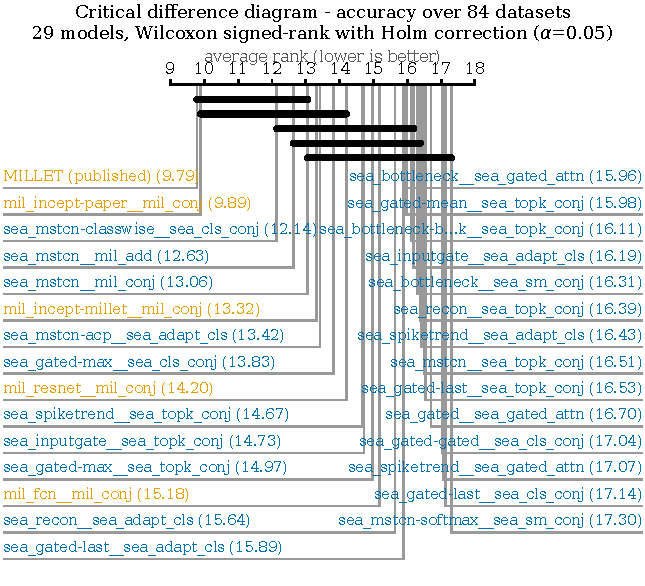
\includegraphics[width=0.85\textwidth]{results/paper_figures/01_main_figures/fig4_critical_difference_accuracy}
  \caption{Critical-difference diagram over the shared \ucr{} datasets. Lower rank is better;
  horizontal bars join models that are not significantly different after Holm correction. Orange
  labels are reproduced baselines, blue are ours. Ranks differ from \Cref{tab:app_ucr} because this
  diagram includes one additional entry --- see the text above.}
  \label{fig:app_cd}
\end{figure}

\subsection{Cost against quality across the whole sweep}
\label{app:pareto}

\begin{figure}[h]
  \centering
  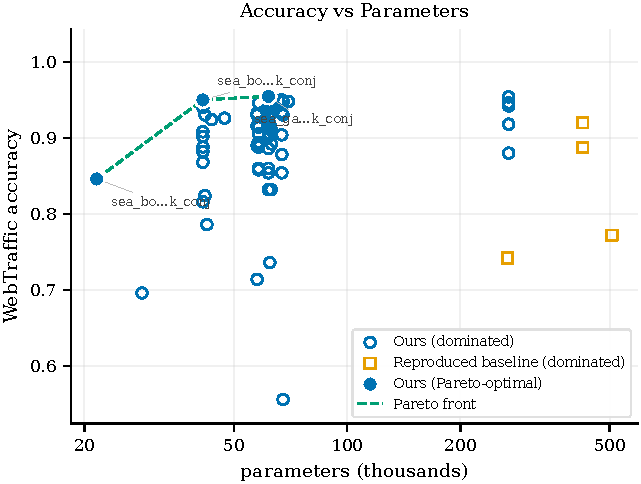
\includegraphics[width=0.6\textwidth]{results/paper_figures/01_main_figures/pareto_web_acc_vs_params}
  \caption{All 72 swept encoder--head combinations (circles) and the reproduced baselines (squares)
  on \webtraffic{}. Filled circles are Pareto-optimal: nothing beats them on both axes at once. The
  baselines occupy the right-hand quarter of the parameter axis without occupying the top of the
  accuracy axis, which is the picture behind \Cref{tab:main,tab:cost}. Labels are abbreviated
  configuration names; \Cref{tab:app_leaderboard} gives them in full.}
  \label{fig:app_pareto}
\end{figure}

\subsection{Relation to published \millet{} results}
\label{app:published}

\begin{table}[h]
\caption{Five ways of obtaining a \millet{} number, and what each is evidence for.}
\label{tab:app_published}
\begin{center}
\small
\begin{tabular}{lcc}
\toprule
\textbf{How obtained} & \webtraffic{} Acc. & \ucr{}-85 Acc. \\
\midrule
Published, mean of 5 seeds \citep{early2024millet} & 0.924 & 0.8445 \\
Published, 5-model ensemble                        & 0.940 & --- \\
Released weights, evaluated in our pipeline        & 0.922 & --- \\
Re-trained here under \emph{their} hyperparameters & 0.920 & 0.8434 \\
Re-trained here under \emph{our} configuration     & 0.887 & 0.8274 \\
\bottomrule
\end{tabular}
\end{center}
\end{table}

The third and fourth rows agree with the first to within $0.4$ and $0.1$ accuracy points, which is
the check that our re-implementation is faithful. The gap between the fourth and fifth rows is
therefore the training budget and nothing else, and it is why the main comparison in \Cref{tab:main}
treats the matched-budget row as the like-for-like baseline while still printing the published-recipe
row as the harder target. We do not reproduce \millet{}'s published AOPCR in this table:
\Cref{sec:res:aopcr} shows it would not be comparable with any value we measured, and quoting it
would contradict our own finding.

\subsection{Full sweep}
\label{app:leaderboard}

\Cref{tab:app_leaderboard} lists all 72 encoder--head combinations, ordered by \webtraffic{}
accuracy. \ucr{} columns are blank where the combination was not run on the archive; those
combinations were screened on \webtraffic{} only, under a fixed compute allocation. One row,
\texttt{seanet\_bottleneck\_adaptive}, completed only 6 of the 85 \ucr{} datasets, so its \ucr{}
values are omitted rather than reported --- a 6-dataset mean is not comparable with an 85-dataset
mean.

% GENERATED by scripts/make_leaderboard_tex.py from
% results/SEA_NET/leaderboard.csv -- do not edit by hand.
{\scriptsize
\setlength{\tabcolsep}{3pt}
\begin{longtable}{rlllcccrr}
\caption{All 72 encoder--head combinations, ordered by \webtraffic{} accuracy. A dash in the
\ucr{} column means the combination was tested on \webtraffic{} only. Pooling heads marked
$^{*}$ are \millet{}'s own, used unchanged.}
\label{tab:app_leaderboard} \\
\toprule
\# & \textbf{Configuration} & \textbf{Encoder} & \textbf{Head} &
Acc. & AOPCR & \ndcg{} & \ucr{}-85 & Params \\
\midrule
\endfirsthead
\multicolumn{9}{l}{\emph{\Cref{tab:app_leaderboard} continued from the previous page.}} \\
\toprule
\# & \textbf{Configuration} & \textbf{Encoder} & \textbf{Head} &
Acc. & AOPCR & \ndcg{} & \ucr{}-85 & Params \\
\midrule
\endhead
\midrule
\multicolumn{9}{r}{\emph{continued on the next page}} \\
\endfoot
\bottomrule
\endlastfoot
1 & \texttt{seanet\_gated\_mean\_topk} & gated & Top-$k$ & 0.955 & 2.23 & 0.750 & 0.8083 & 61{,}740 \\
2 & \texttt{seanet\_conjunctive} & plain & conjunctive* & 0.954 & 1.50 & 0.698 & 0.8238 & 269{,}083 \\
3 & \texttt{seanet\_gated\_max\_topk} & gated & Top-$k$ & 0.952 & 2.27 & 0.719 & 0.8108 & 61{,}740 \\
4 & \texttt{seanet\_topk\_nofocus} & bottleneck & Top-$k$ & 0.950 & 2.30 & 0.765 & --- & 41{,}324 \\
5 & \texttt{seanet\_spiketrend\_topk} & spike/trend & Top-$k$ & 0.950 & 2.32 & 0.756 & 0.8089 & 67{,}020 \\
6 & \texttt{seanet\_inputgate\_mschan} & ms-channels & Top-$k$ & 0.948 & 2.32 & 0.757 & --- & 69{,}768 \\
7 & \texttt{seanet\_gated\_mschan} & ms-channels & Top-$k$ & 0.948 & 2.22 & 0.717 & --- & 67{,}592 \\
8 & \texttt{seanet\_bottleneck\_topk} & bottleneck & Top-$k$ & 0.947 & 2.62 & 0.772 & 0.8097 & 41{,}324 \\
9 & \texttt{seanet\_recon\_adaptive} & recon & adaptive & 0.946 & 2.60 & 0.768 & 0.8140 & 62{,}935 \\
10 & \texttt{seanet\_inputgate\_topk} & input-gated & Top-$k$ & 0.946 & 2.80 & 0.748 & 0.8131 & 58{,}092 \\
11 & \texttt{seanet\_classwise} & plain & class-wise & 0.946 & 1.72 & 0.686 & 0.8292 & 269{,}164 \\
12 & \texttt{seanet\_gated\_max} & gated & class-wise & 0.944 & 1.89 & 0.592 & 0.8237 & 61{,}740 \\
13 & \texttt{seanet\_gated\_last\_topk} & gated & Top-$k$ & 0.942 & 2.31 & 0.748 & 0.8015 & 61{,}740 \\
14 & \texttt{seanet} & plain & additive* & 0.942 & 1.58 & 0.729 & 0.8298 & 269{,}083 \\
15 & \texttt{seanet\_gated\_last} & gated & class-wise & 0.942 & 2.52 & 0.742 & 0.7888 & 61{,}740 \\
16 & \texttt{seanet\_recon\_topk} & recon & Top-$k$ & 0.940 & 2.51 & 0.698 & 0.8063 & 62{,}925 \\
17 & \texttt{seanet\_topk\_k025} & bottleneck & Top-$k$ & 0.940 & 2.65 & 0.733 & --- & 41{,}324 \\
18 & \texttt{seanet\_bottleneck\_softmax} & bottleneck & softmax & 0.940 & 1.68 & 0.740 & 0.8106 & 41{,}325 \\
19 & \texttt{seanet\_gated\_last\_adaptive} & gated & adaptive & 0.938 & 2.39 & 0.793 & 0.8029 & 61{,}750 \\
20 & \texttt{seanet\_spiketrend\_adaptive} & spike/trend & adaptive & 0.934 & 1.91 & 0.747 & 0.8010 & 67{,}030 \\
21 & \texttt{seanet\_recon\_softmax} & recon & softmax & 0.932 & 1.64 & 0.723 & --- & 62{,}926 \\
22 & \texttt{seanet\_slim\_topk} & plain & Top-$k$ & 0.932 & 2.69 & 0.778 & 0.8093 & 57{,}580 \\
23 & \texttt{seanet\_bottleneck\_gatedattn} & bottleneck & gated-attn & 0.930 & 2.23 & 0.741 & 0.8146 & 41{,}844 \\
24 & \texttt{seanet\_spiketrend\_gatedattn} & spike/trend & gated-attn & 0.930 & 1.59 & 0.721 & 0.8039 & 67{,}540 \\
25 & \texttt{seanet\_gated} & gated & class-wise & 0.930 & 2.41 & 0.637 & 0.7900 & 61{,}740 \\
26 & \texttt{seanet\_slim\_adaptive} & plain & adaptive & 0.930 & 2.45 & 0.793 & --- & 57{,}590 \\
27 & \texttt{seanet\_bottleneck\_mschan} & ms-channels & Top-$k$ & 0.926 & 2.24 & 0.777 & --- & 47{,}176 \\
28 & \texttt{seanet\_bottleneck\_mschan\_lean} & ms-channels & Top-$k$ & 0.924 & 2.76 & 0.735 & --- & 43{,}576 \\
29 & \texttt{seanet\_gated\_last\_softmax} & gated & softmax & 0.920 & 1.99 & 0.738 & --- & 61{,}741 \\
30 & \texttt{millet\_paper} & InceptionTime & conjunctive* & 0.920 & 13.27 & 0.661 & 0.8434 & 423{,}707 \\
31 & \texttt{seanet\_acp} & plain & adaptive & 0.918 & 1.61 & 0.619 & 0.8134 & 269{,}174 \\
32 & \texttt{seanet\_gated\_last\_gatedattn} & gated & gated-attn & 0.918 & 1.35 & 0.757 & 0.8048 & 62{,}260 \\
33 & \texttt{seanet\_slim} & plain & class-wise & 0.916 & 2.48 & 0.719 & --- & 57{,}580 \\
34 & \texttt{seanet\_gated\_max\_softmax} & gated & softmax & 0.914 & 1.88 & 0.776 & --- & 61{,}741 \\
35 & \texttt{seanet\_inputgate} & input-gated & class-wise & 0.914 & 2.48 & 0.715 & --- & 58{,}092 \\
36 & \texttt{seanet\_gated\_mean\_softmax} & gated & softmax & 0.912 & 2.09 & 0.765 & --- & 61{,}741 \\
37 & \texttt{seanet\_recon} & recon & class-wise & 0.910 & 2.50 & 0.680 & --- & 62{,}925 \\
38 & \texttt{seanet\_topk\_k100} & bottleneck & Top-$k$ & 0.908 & 2.44 & 0.722 & --- & 41{,}324 \\
39 & \texttt{seanet\_gated\_max\_adaptive} & gated & adaptive & 0.906 & 2.07 & 0.729 & --- & 61{,}750 \\
40 & \texttt{seanet\_inputgate\_adaptive} & input-gated & adaptive & 0.905 & 2.65 & 0.732 & 0.8153 & 58{,}102 \\
41 & \texttt{seanet\_spiketrend} & spike/trend & class-wise & 0.904 & 2.15 & 0.699 & --- & 67{,}020 \\
42 & \texttt{seanet\_bottleneck} & bottleneck & class-wise & 0.902 & 2.57 & 0.733 & --- & 41{,}324 \\
43 & \texttt{seanet\_gated\_mean} & gated & class-wise & 0.902 & 2.49 & 0.714 & --- & 61{,}740 \\
44 & \texttt{seanet\_inputgate\_softmax} & input-gated & softmax & 0.894 & 1.64 & 0.696 & --- & 58{,}093 \\
45 & \texttt{seanet\_slim\_gatedattn} & plain & gated-attn & 0.894 & 2.30 & 0.714 & --- & 58{,}100 \\
46 & \texttt{seanet\_recon\_attnmax} & recon & attn-max & 0.892 & 2.32 & 0.725 & --- & 62{,}935 \\
47 & \texttt{seanet\_slim\_softmax} & plain & softmax & 0.890 & 1.83 & 0.705 & --- & 57{,}581 \\
48 & \texttt{seanet\_slim\_gatedattn} & gated & attention* & 0.888 & 2.40 & 0.710 & --- & 58{,}100 \\
49 & \texttt{seanet\_topk\_k005} & bottleneck & Top-$k$ & 0.888 & 2.29 & 0.715 & --- & 41{,}324 \\
50 & \texttt{millet} & InceptionTime & conjunctive* & 0.887 & 2.57 & 0.677 & 0.8274 & 423{,}707 \\
51 & \texttt{seanet\_gated\_max\_attnmax} & gated & attn-max & 0.886 & 1.12 & 0.575 & --- & 61{,}750 \\
52 & \texttt{seanet\_topk\_k050} & bottleneck & Top-$k$ & 0.882 & 3.11 & 0.732 & --- & 41{,}324 \\
53 & \texttt{seanet\_softmax} & plain & softmax & 0.880 & 1.02 & 0.605 & 0.8131 & 269{,}165 \\
54 & \texttt{seanet\_spiketrend\_softmax} & spike/trend & softmax & 0.878 & 1.43 & 0.665 & --- & 67{,}021 \\
55 & \texttt{seanet\_bottleneck\_adaptive} & bottleneck & adaptive & 0.868 & 1.97 & 0.680 & --- & 41{,}334 \\
56 & \texttt{seanet\_slim\_dualstream} & plain & dual-stream & 0.860 & 2.40 & 0.745 & --- & 58{,}101 \\
57 & \texttt{seanet\_gated\_mean\_adaptive} & gated & adaptive & 0.860 & 2.24 & 0.731 & --- & 61{,}750 \\
58 & \texttt{seanet\_inputgate\_attnmax} & input-gated & attn-max & 0.858 & 2.15 & 0.700 & --- & 58{,}102 \\
59 & \texttt{seanet\_spiketrend\_attnmax} & spike/trend & attn-max & 0.854 & 1.65 & 0.644 & --- & 67{,}030 \\
60 & \texttt{seanet\_gated\_last\_attnmax} & gated & attn-max & 0.854 & 1.78 & 0.668 & --- & 61{,}750 \\
61 & \texttt{seanet\_bottleneck\_shallow} & bottleneck & Top-$k$ & 0.846 & 2.82 & 0.624 & --- & 21{,}548 \\
62 & \texttt{seanet\_gated\_mean\_attnmax} & gated & attn-max & 0.832 & 1.67 & 0.704 & --- & 61{,}750 \\
63 & \texttt{seanet\_gated\_pyramid} & ms-pyramid & Top-$k$ & 0.832 & 0.98 & 0.591 & --- & 62{,}781 \\
64 & \texttt{seanet\_bottleneck\_dualstream} & bottleneck & dual-stream & 0.824 & 2.04 & 0.652 & --- & 41{,}845 \\
65 & \texttt{seanet\_bottleneck\_attnmax} & bottleneck & attn-max & 0.816 & 1.74 & 0.610 & --- & 41{,}334 \\
66 & \texttt{seanet\_bottleneck\_pyramid} & ms-pyramid & Top-$k$ & 0.786 & 1.03 & 0.569 & --- & 42{,}365 \\
67 & \texttt{resnet} & ResNet & conjunctive* & 0.772 & 2.95 & 0.554 & 0.8146 & 506{,}331 \\
68 & \texttt{fcn} & FCN & conjunctive* & 0.742 & 3.83 & 0.533 & 0.8141 & 267{,}035 \\
69 & \texttt{seanet\_gated\_last\_dualstream} & gated & dual-stream & 0.736 & 1.95 & 0.637 & --- & 62{,}261 \\
70 & \texttt{seanet\_slim\_attnmax} & plain & attn-max & 0.714 & 1.63 & 0.532 & --- & 57{,}590 \\
71 & \texttt{seanet\_bottleneck\_mschan\_pyramid} & ms-pyramid & Top-$k$ & 0.696 & 2.17 & 0.653 & --- & 28{,}441 \\
72 & \texttt{seanet\_spiketrend\_dualstream} & spike/trend & dual-stream & 0.556 & 1.64 & 0.510 & --- & 67{,}541 \\
\end{longtable}}



\end{document}
